%%
% TUM Corporate Design LaTeX Templates
% Based on the templates from https://www.tum.de/cd
%
% Feel free to join development on
% https://gitlab.lrz.de/tum-templates/templates
% and/or to create an issue in case of trouble.
%
% tum-article class for scientific articles, reports, exercise sheets, ...
%
%%

\documentclass[twocolumn]{tum-article}
%\documentclass[twocolumn, german]{tum-article}
%\documentclass[times, twocolumn]{tum-article}
%\documentclass[times]{tum-article}
%\documentclass{tum-article}

%\usepackage{lipsum}
\usepackage{listings}

\title{Analysis of the 2014 Passenger Flight Network}
\author{Felix Paul Niemeyer\authormark{1},
	Saicharan Kumar\authormark{2}}
% Author 3\authormark{1}\orcid{0000-0000-0000-0000}}

% if too long for running head
\titlerunning{TUM Article}
\authorrunning{Author 1 et al.}

%\email{niemeyer.felix@tum.de}

\affil[1]{felix.niemeyer@tum.de, MiM}
\affil[2]{saicharan.kumar@tum.de, MiM}

\date{Received: 19.02.2020 - This is work in progress}

\begin{document}

\maketitle

\begin{abstract}
	In this case study we are looking at a dataset about air travel in 2014. We implement some mechanisms to clean the data, as well as mechanisms to enrich this dataset with information we query from wikidata. We estimate some missing data. Starting from there, we analyze some network characteristics for the whole network as well as airline-specific sub-networks. We compare airline-specific networks and find relations between their network's characteristics and their business model. We propose one metric that plays a role in forcasting whether a cooperation between two airlines is advantageous and use this metric to generate an alliances landscape. We compare it's predictive correctness to the real world by looking at the formation of Vanilla Airlines which occured in the year after the one our data stems from. 
\end{abstract}

\section{Data Description}
The network analysis is based on dataset from openflights.org. 
It describes passenger flight connections between airports in the year 2014. 
The data includes, which airline each connection is operated by.
The data comes in three tables: airports, routes and airlines. 
The airports table has entries for every airport with the following useful information: \\
- airport id\\
- iata and icao codes\\
- geographic coordinates\\
- country and region\\

The routes table lists an entrie for each connection between two airports that was operated by an airline somewhen in the year 2014. It does not contain any information about flight frequencies or passenger volume. The airline table lists airlines associated with their name and some information we do not need like country or callsign. \\

We are loading these files into an sqlite database for easier handling. 
We apply some queries for cleaning the data, e.g. removing routes operated by unknown airlines or filling in airport ids in routes where only iata or icao code is used to refer to a source or destination airport. \\

All the data-setup can be acomplished by running a single script.
This script and also all other code we have written for this project can be found in a public repository on GitHub\cite{repository}.

\section{Data Enrichment \& Estimation}
After cleaning up the data, there are 3139 airports. 
Interpreting the data as a graph gives us a multiedge directed graph).
Looking at the degree distribution in Figure~\ref{fig:degree_distribution}, the alternating characteristic of degrees strikes the eye. It comes from the fact, that it's very uncommon for a connection between airports to exist only in one direction. Thus, there is much fewer nodes with odd degrees than than with even degrees. 

When we disregard odd degress, the seemingly linear distribution on a log log scale becomes apparent. Using least square (scipy.optimize.curve\_fit), we optimize paramters $c$ and $\gamma$ as you can see in Figure~\ref{fig:degree_distribution_curves}

\begin{figure}
	\centering
	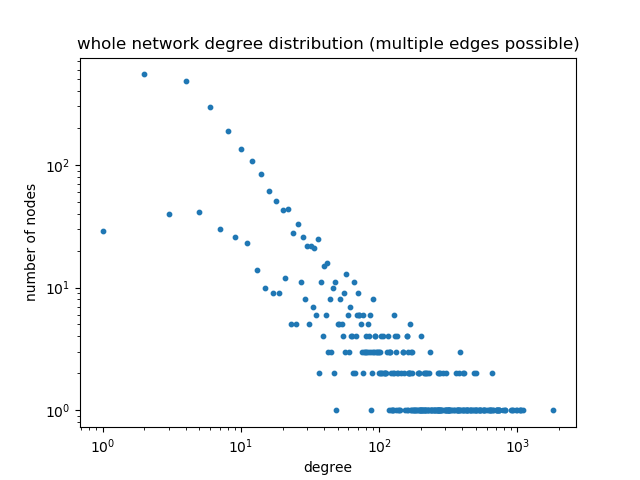
\includegraphics[width=76mm]{imgs/results/degree_distribution_incl_odd_degrees.png}
	\caption{
The degree distribution of the network on a log log scale }
	\label{fig:degree_distribution}
\end{figure}

\begin{figure}
	\centering
	\includegraphics[width=76mm]{imgs/results/degree_distribution_curve_manual.png}
	\caption{
Looking at even degrees only. Trying least square curve fitting to find suitable parameters for power law distribution function $f(x) = a * x^{-\gamma}$}
	\label{fig:degree_distribution_curves}
\end{figure}

Besides the main subgraph, that includes 3113 nodes, there are 6 small disconnected ones with only a couple of nodes.
One with 10 nodes for example Figure~\ref{fig:new_caledonia}, consists only of airports that are located in New Caledonia, an archipelago in the Pacific Ocean. 
\begin{figure}
	\centering
	\includegraphics[width=76mm]{imgs/new-caledonia-subgraph.png}
	\caption{Airports of New Caledonia drawn on a map}
	\label{fig:new_caledonia}
\end{figure}

In order to enable us to do more meaningful analysis, we enrich the dataset with additional information. We chose the airport patronage and found out, that we can get this data from Wikidata. 
For 1956 of the 3139 airports from the dataset, we can find patronage data from Wikidata. 
We need to distinguish between monthly and yearly values and we extrapolate 2014 data from close years in case no data for the year 2014. 
In order to populate the remaining nodes with reasonable patronages as well, we tried different techniques. 
First we used data about runway surfaces that we found on ourflights.org. We summed up the surfaces of runways for every airport and then calculated the average ratio between total runway surface area and patronage of airports where both data points were present, in order to predict patronage for airports without patronage data but with runway surface data based on this average ratio. For the still remaining >1000 airports without patronage we would then apply a default value that equals the avg of the smallest 1\% of airports with patronage data from Wikidata. 
The runway data turned out to be very unclean and unreliably. Water runways and other quirks were distorting the predictions. 

Inspired by Prof. Ikonnikova advice during the presentation we switched to estimating the remaining airport patronages by looking at neighboring airports with patronage data.

\begin{lstlisting}[language=Python, caption=Patronage Estimation]
G = loadEntireNetwork()
pr = -1 #previous remaining
r = 0   #remaining
while r != pr:
  pr = r
  r = 0
  ep = {} #estimated patronages
  for apid in G.nodes:
    node = G.nodes[apid]
    if node["patronage"] == None:
      neighbors = G.neighbors(apid) 
      deg = G.degree(apid)
      sum = 0
      count = 0
      for nid in neighbors: 
        n = G.nodes[nid]
        npatr = n["patronage"]
        ndeg = G.degree(nid) 
        if npatr != None: 
          sum += deg * npatr / ndeg
          count += 1
      if count == 0:
        r += 1
      else:
        avg = sum / count
        ep[apid] = avg 
  for apid in ep: 
    node = G.nodes[apid]
    node["patronage"] = ep[apid]
\end{lstlisting}

This seccond approach yields much nicer estimations, as we will see after estimating the flows between airports. 

The flows are estimated by choosing reasonable initial values and then applying corrections iteratively to approach a situation where the sum of the estimated flows for each airport equal its patronage value.
The average initial values for an edge between airport a and b is chosen as: \footnote{hmm, vielleicht auch nicht den avg, sondern den total flow zwischen den airports so berechenen - ich mein, das hab ich ja gemacht!}

$avgFlow_{ab} = $

$\dfrac{patronage(a) * patronage(b)}{degree(a) * degree(b)}$ 

Remember that we are handling a multiedge directed graph here. There may be multiple edges between two airports pointing in different directions and/or operated by different airlines.
We could assume an equal distribution of the flows among the edges. But we chose trying to be closer to reality by weighting the flow of an edge between two airports $a$ and $b$, that is operated by airline $o$, by the geometric mean of the number of edges airline $o$ operates at airport $a$ and number of edges airline $o$ operates at airport $b$: 

$flow_{ab} = $

$avgFlow_{ab} * (|E_{ab}|+|E_{ba}|) * weight_{abo}$

Where $|E_{ab}|$ is the number of directed edges from $a$ to $b$ and

$weight_{abo} = $

$\dfrac{\sqrt{degree_{o}(a) * degree_{o}(b)}}{\displaystyle\sum_{l \in L \land c,d \in \{a,b\} \land c \neq d}(\sqrt{degree_{l}(c) * degree_{l}(d)})}$  

The ratios we choose here will stay intact over the course of the iterations in the next part of the algorithm. 

<describe iteration step>

<Show results, compare runway to neighbor based estimation>

The complete algorithm for passenger flow estimation is too long for beeing included in this document. You can find it in the repository: ./scripts/estimate-passenger-flows.py

After estimating missing patronage data by looking at neighboring airports patronages, 14 airports without patronage remain. These must be in airports in disconnected subgraphs, because the algorithm would eventually reach them and assign a patronage otherwise. Investigations confirm that. We disregard these few dataless airports from disconnected subgraphs in the following analysises and thus end up with a network of 3125 airports. 


\section{Basic Network Analysis}
Initially, we would like to analyse the entire worldwide airline network, and provide some insights regarding the airline industry.
Since a particular route could be provided by multiple Airline Companies, the final network that we come up with is a Multiple Directed Network.
The attributes of each edge in this network included both the geometrical distance and the average passenger flow of that route (edge). 
As we can see from the Table~\ref{Tab:distance_metrics}, the diameter of the entire network is given along with the Total Distance of the routes and the Average Distance of routes in a network.  

\begin{center}
\begin{table}[ht]	
 \begin{tabular}{| c | c | c |}
 \hline
 Diameter & Total Distance & Average Distance \\ [0.5ex]
 \hline
 18834 & 126681574 & 1889.72 \\
 \hline
 \end{tabular}
\caption{Distance Metrics of the Network}
\label{Tab:distance_metrics}	 
\end{table}
\end{center}

We currently do not have the ability to calculate centrality parameters like Eigenvector, Closeness or Betweenness Centrality for a Multidirected Graph. So we will be mainly looking at Degree Centrality of the entire network as shown in Figure~\ref{fig:degree_centrality}.
This is because Degree Centrality is the only Centrality available for Multiple Directed Graphs.

\begin{figure}
        \centering
        \includegraphics[width=80mm]{imgs2/results/degree_centrality_whole_network.png}
        \caption{
The degree centrality of the entire network}
        \label{fig:degree_centrality}
\end{figure}

The degree centrality is given by the formula:
\begin{equation}
	Degree Centrality=d_i/(n-1)
\end{equation}

Just by analysing the graph, we can say that the degree centrality distributrion is following the Power Law Distribution. 

\section{Airline Subnetwork Analysis \& Comparison}
W

\section{Airline Cooperation Opportunity}

The possibility to provide convenient on-line connections to clients is an important factor that drives welfare gains through ailine cooperation according to E. E. Bailey and D. Liu \cite{airline_consolidation_and_consumer_welfare}.

\section{Reality Check: Vanilla Airlines}


\section*{Acknowledgements}


\bibliographystyle{IEEEtran}
\bibliography{literature}

\end{document}
